\chapter{Lösungsvorschläge}
In diesem Kapitel werden Lösungsvorschläge zur Beseitigung der in Kapitel 4 beschriebenen Probleme formuliert.
\section{Implementierung eines Ruby on Rails Content Repository}

Die in den analysierten WCMS umgesetzten Implementierungen der Erweiterungsentwicklung verstoßen zum Teil gegen das in Rails gebotene Prinzip des DRY (vgl. Kapitel \ref{dryverstoss}). Eine konzeptionelle Änderung innerhalb dieses Systembereiches hätte somit Auswirkungen auf die gesamte WCMS-Infrastruktur der Inhaltsspeicherung. Dennoch soll hier der mögliche Lösungsansatz eines Content Repository konzeptionell vorgestellt werden.


\subsection{Idee und Konzept}

Heutige Webanwendungen (u.a. auch Web Content Management Systeme) benötigen neben der klassischen Speicherung von Daten zahlreiche zusätzliche Daten-Management-Funktionalitäten. Ein Content Repository (CR) soll dieser Entwicklung Rechnung tragen und definiert daher ein abstraktes Datenmodell zur Datenspeicherung und zusätzliche Servicefunktionalitäten, die häufig von content-orientierten Anwendungen verwendet werden. Ein Content Repository stellt somit u.a. folgendes Leistungsspektrum bereit:

\begin{itemize}
\item
Speicherung strukturierter und unstrukturierter Daten (z.B. Binär- und Textformate oder Metadaten),
\item
Möglichkeiten der Zugangskontrolle
\item
Möglichkeiten der Sperrung (Locking)
\item
Durchführung von Transaktionen
\item
Versionierungsmechanismen
\item
Überwachung von Daten
\item
Volltextsuche
\end{itemize}

Der Zugriff auf das Content Repository wird dabei durch eine API genau definiert und garantiert somit einen definierten Zugriff auf die zusäzlichen Funktionalitäten. Andere Entwickler können auf das Content Repository und seine Zusatzfunktionen kontrolliert zugreifen, ohne etwas über die Infrastruktur und seine Implementierungsdetails zu wissen. Intern greift das Content Repository auf andere Technologien und Infrastrukturen zurück, um die geforderten Funktionalitäten abzubilden\footnote{Das im folgenden beschriebene Java Content Repository Jackrabbit verwendet in seiner Standardkonfiguration z.B. WebDAV zur Speicherung von Daten sowie Apache Lucene zur Realsierung der Suchindexierung.}.

Im Bereich der Java Enterprise Content Management Systeme werden Content Repositories bereits erfolgreich eingesetzt. Namhafte Beispiele sind dabei das kommerzielle ECMS CQ5 und CRX\footnote{Nach der Übernahme von Day Inc. durch Adobe im Sommer 2010 wird das angebotene Content Management System CRX als Adobe Projekt weitervertrieben.} von Adobe und das u.a. als Open Source Software verfügbare Alfresco ECMS\footnote{Informationen zu Alfresco und dem Content Repository: \href{http://www.alfresco.com/products/platform/}{http://www.alfresco.com/products/platform/}}.
Innerhalb der PHP-Entwicklergemeinde wird ebenfalls gerade an der Umsetzung eines auf PHP basierten Content Repositories gearbeitet. Initiatoren sind dabei vor allem die Typo3 Association mit einer Implementierung innerhalb des neuen Web Content Management Systems Typo3 5.0\footnote{Das TYPO3CR ist als eigenständiges Paket im PHP-FLOW3-Framework verfügbar und ein zentraler Bestandteil von Typo3 5.0}.


\subsection{JCR-Das Java Content Repository}

Unter der Leitung von David Nüscheler der Firma Day Software wurde 2005 die erste Version einer Implementierung und API Spezifikation eines Java Content Repository veröffentlicht\footnote{Die Entwicklung ging im Java Specification Request (JSR) 170 als offizieller Standard in die Programmiersprache Java ein. Momentan wird an der Veröffentlichung der Version 2.0 des Standards gearbeitet(JSR-283).}. Die umgesetzte Referenzimplementierung wurde später unter der Leitung der Apache Foundation als Open Source Projekt Jackrabbit\footnote{Projektseite: \href{http://jackrabbit.apache.org/}{http://jackrabbit.apache.org/}} der Öffentlichkeit zur Verfügung gestellt.

Zur Speicherung der Inhalte definiert das Java Content Repository ein einfaches hierarchisches Datemmodell, das folgende Objektstruktur aufweist:


\begin{figure}[!h]
\begin{center}
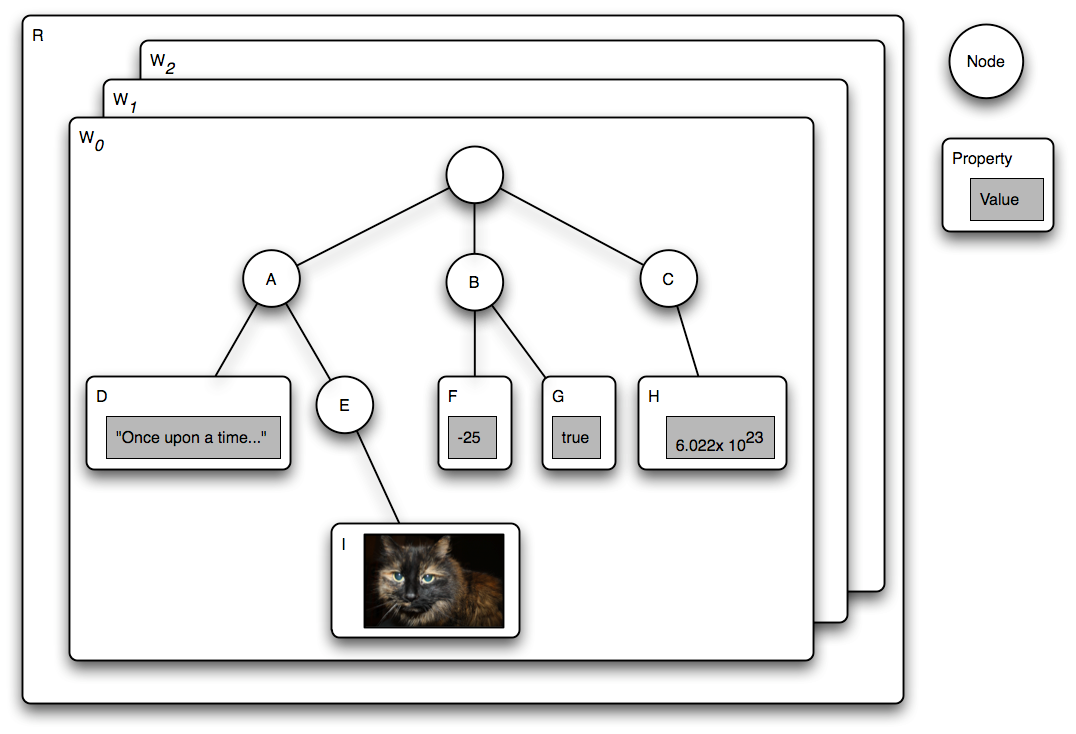
\includegraphics[scale=0.3]{images/repository/repository_diagramm.png}
\caption{JCR-Datenmodell}
\label{jcrdatenmodell}
\end{center}
\end{figure}



\begin{description}
\item[Workspace]\mbox{~}\\*
Ein JCR-Repository besteht aus einem oder mehreren Workspaces (Arbeitsbereichen), die jeweils mehrere Items in einer Baumstruktur beliebiger Tiefe verwalten können. Jeder Workspace lässt sich durch einen Namen eindeutig identifizieren (W\textsubscript{0}, W\textsubscript{1}, W\textsubscript{2}) und enthält mindestens ein Item (root node).
\item[Item]\mbox{~}\\*
Ein Item kann entweder ein Node (Knoten) oder ein Property (Eigenschaft) sein.
\item[Node]\mbox{~}\\*
Knoten (Nodes) eines Workspaces bilden die Struktur der zu speichernden Daten ab.
Ein Knoten kann daher keine oder weitere andere Kinderknoten (child notes) enthalten.
\item[Property]\mbox{~}\\*
Eine Property kann keine anderen Items beinhalten, aber dafür den Inhalt in Form von sogenannten Values abspeichern. Dabei kann ein Property-Node keine oder mehrere Values beinhalten.
\end{description}




\subsection{Umsetzungsvarianten innerhalb von Ruby on Rails}

Durch die Verfügbarkeit eines Ruby-Interpreter in der Programmiersprache Java (jruby\footnote{Projektseite: \href{http://jruby.org/}{http://jruby.org/}}) ergeben sich für die Umsetzung in Ruby on Rails folgende 2 Möglichkeiten:

\begin{itemize}
\item
Verwendung der Open Source Java Implementierung Jackrabbit und Spezifikation einer API zur Nutzung dieser innerhalb von Rails. Erste Implementierungsversuche und Demonstrationsanwendungen wurden bereits erstellt\footnote{Eine Rails2-Demo-Anwendung ist unter folgender Internetseite erreichbar: \href{https://github.com/wpc/jcr-rails-demo}{https://github.com/wpc/jcr-rails-demo}. Sie zeigt dabei lediglich das konzeptionelle Grundgerüst zur Umsetzung des Content Repository auf.}.
\item
Erstellung einer eigenständigen, komplett auf Ruby und dem Rails Framework basierenden Referenzimplementierung und API nach dem Vorbild des Java Content Repository
\end{itemize}


\subsection{Vorteile für die gewählten Ruby on Rails WCMS}

Die Umsetzung eines Content Repository in Ruby kann für die bestehenden Web Content Management Systeme folgende Vorzüge bringen:

\begin{itemize}
\item Beseitigung des DRY-Verstosses bei den untersuchten Rails-WCMS, da die Inhalte in dem durch das Content Repository zur Verfügung gestellten hierarchischen Datenmodell gespeichert werden können.
\item
Wegfall der bisher notwendigen Datenbankmigrationen und zusätzlichen Datenbanktabellen, da das Content Repository die gesamte Infrastruktur bereitstellt und die Speicherung der Daten übernimmt.
\item Vereinfachung des Zugriffs auf Inhalte innerhalb verschiedener Systeme durch Verwendung einer definierten API
\item Fehlende Webpublishing-Funktionalitäten der existierenden Rails WCMS können durch eine Implementierung eines Content Repository als Infrastruktur allgemein zur Verfügung gestellt werden (z.B. Versionierung, Suchfunktionen).
\item Durch die im JCR-Standard festgelegten Import- und Exportfunktionen kann ein Austausch der Inhalte zwischen verschiedenen Web Content Management Systemen ermöglicht werden.
\item Ein Content Repository kann als Erweiterung auch von anderen Rails-Anwendungen verwendet werden, die mit verschiedenartig strukturierten Inhalten umgehen müssen.
\end{itemize}



\section{Übertragung des Typo3 5.0 Phoenix User-Interfaces in Rails 3.1}
Content Management Systeme erfordern bei steigender Funktionalität ein entsprechend komplexeres Nutzer-Interface. Die sinnvolle Realisierung entsprechender Oberflächen ist mit der u.a. in Refinery CMS gewählten Generierung von HTML-Views und einzelnen JavaScript-Dateien nur noch schwer möglich. Zur Umsetzung solcher Projekte empfiehlt sich daher der Einsatz alternativer Technologien.
Die neue Version 5.0 des PHP basierten Web Content Management Systems Typo3 greift bei der Generierung der gesamten Backend-Oberfläche auf das Java Script Frameworks Ext JS 4\footnote{Informationen und Download: \href{http://www.sencha.com/}{http://www.sencha.com/}} zurück. Es ermöglicht durch Kombinierung vorgefertigter Elemente eine schnelle Erstellung komplexer Oberflächen\footnote{Beispielanwendungen: \href{http://dev.sencha.com/deploy/ext-4.0.0/examples/}{http://dev.sencha.com/deploy/ext-4.0.0/examples/}}.
Die Veröffentlichung des Typo3-Projektes unter der GPLv3-Lizenz macht eine Weiternutzung der in der Version 5.0 geplanten Oberfläche generell möglich. Im folgenden sollen daher die notwendigen Schritte zur Integrierung des Typo3 5.0 User-Interfaces in eine Rails 3.1 Anwendung beschrieben werden.

\subsection{Typo3 5.0}
Die Entwicklung von Typo3 5.0 befindet sich noch in einer frühen Phase. Interessenten können jedoch bereits Entwicklerversionen in Form sogenannter Sprint Releases herunterladen und testen. Neben einem Download-Paket\footnote{Komponenten-Download: \href{http://flow3.typo3.org/typo3-phoenix/}{http://flow3.typo3.org/typo3-phoenix/}} auf der Projektseite von Typo3 wird zusätzlich eine aktuelle Version von Typo3 als Live-Demo\footnote{Demoseite: \href{http://phoenix.demo.typo3.org/}{http://phoenix.demo.typo3.org/}} angeboten. Die Zugangsdaten zum Backend können im Frontend der Seite mit Hilfe eines Formulars erzeugt werden.


\begin{figure}[!h]
\begin{center}
\label{fig.typo3frontend}
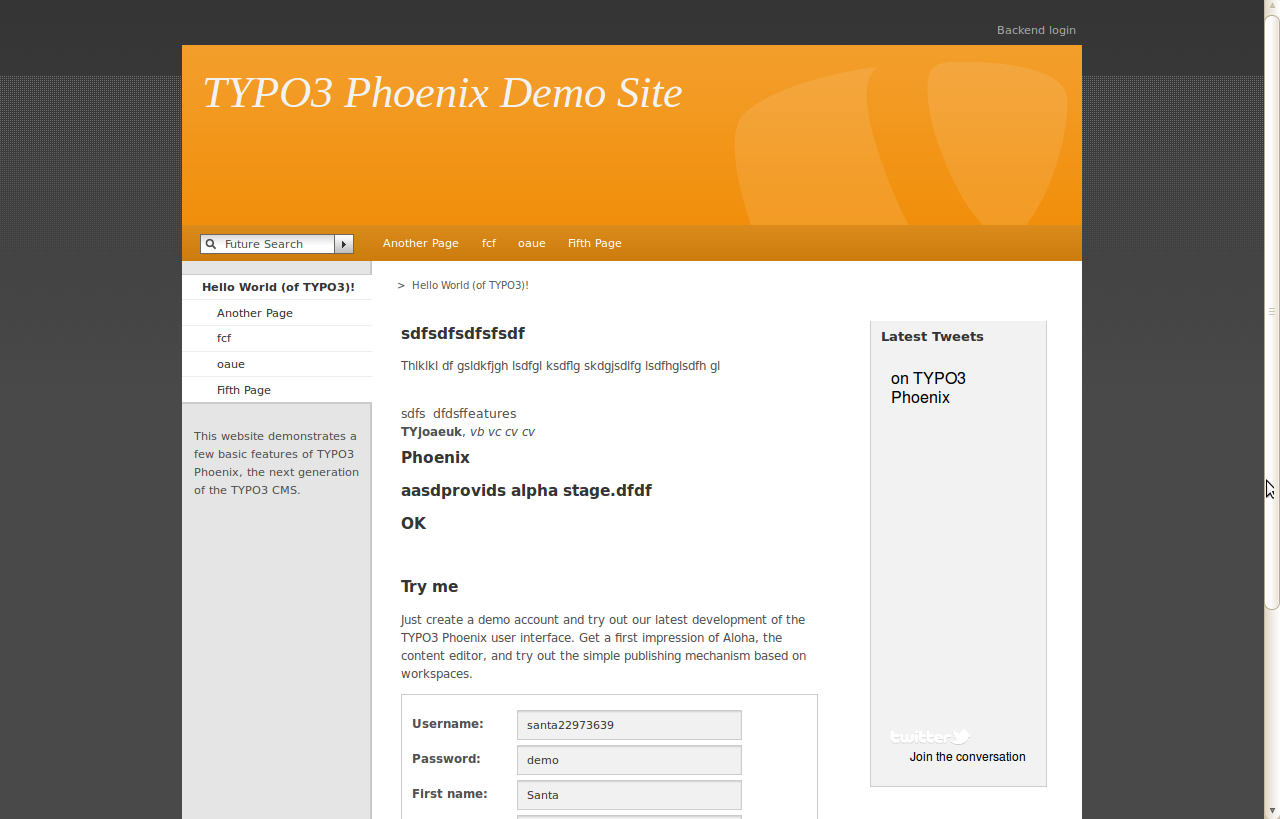
\includegraphics[scale=0.239]{images/typo3/frontend.png}
\caption{Frontend-Ansicht der Typo3 5.0 Sprint Release 6 Demoversion}
\end{center}
\end{figure}


\begin{figure}[!h]
\begin{center}
\label{fig.typo3backend}
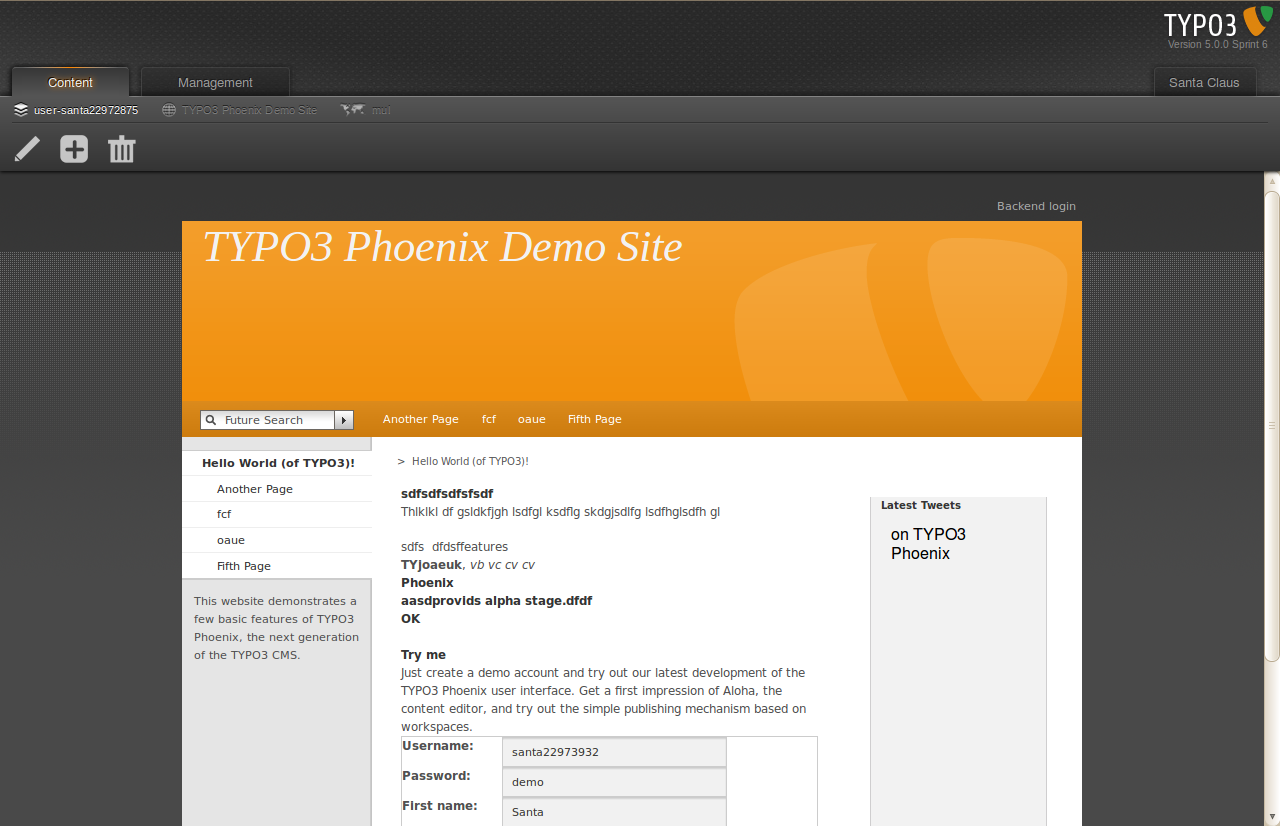
\includegraphics[scale=0.239]{images/typo3/backend.png}
\caption{Backend-Ansicht der Typo3 5.0 Sprint Release 6 Demoversion}
\end{center}
\end{figure}
\newpage
Das in der Demoversion umgesetzte Nutzer-Interface repräsentiert nur einen Teil der für Typo3 5.0 geplanten Oberfläche und Komponenten\footnote{Bilder und ausführliche Erläuterungen zur neuen Typo3 5.0 Oberfläche sind unter folgender Adresse zu finden: \href{http://typo3.org/teams/usability/t35ui/}{http://typo3.org/teams/usability/t35ui/}}. U.a. sind folgende Bestandteile bereits umgesetzt wurden:
\begin{itemize}
\item
Login-Seite zur Anmeldung im Backend von Typo3 5.0
\item
Content-Modul im Backend mit integrierter Vorschau der aktuell ausgewählten Seite und beschränkten Möglichkeiten der Inhaltsbearbeitung mit Hilfe des für Typo3 5.0 geplanten Aloha-Editors
\item
Management-Modul zur Verwaltung der im System angelegten Seiten in Form einer Baumstruktur
\item
Dashboard des angemeldeten Nutzers mit Auflistung der editierten Inhalte
\end{itemize}


\subsection{Ext JS und Ext Direct}

Das Typo3-User-Interface setzt bei der Kommunikation zwischen den einzelnen Interface-Komponenten und dem Server auf die Nutzung von Ext Direct. Ext Direct beschreibt dabei einen in Ext JS definierten Sprachstandard, mit dessen Hilfe serverseitige Funktionen clientseitig per Javascript aufgerufen werden können.
Für ein besseres Verständnis wird in Abbildung \ref{extinvoke} eine im jQuery Framework formulierte Ajax-Anfrage und der entsprechende Ext Direct Ausdruck gegenübergestellt.

\begin{lstlisting}[label=extinvoke, caption=Ajax-Anfrage an einen Server im jQuery-Framework]

// jQuery Ajax Request
$.ajax({
  url: '/ajax?ajaxID=MyController_myMethod&amp;parameter1=someValue',
   success: function( data ) {
    alert(data);
    }
  }
});

// Ext Direct Aufruf
Namespace.MyController.myMethod("some_Value", function(data, e) {
  	alert(data);
});

\end{lstlisting}

Beide Javascript-Beispiele resultieren in einer asynchronen Ajax-Anfrage, die die entsprechende Methode serverseitig aufruft. Für Ext Direct ergeben sich jedoch folgende zusätzliche Vorteile:

\begin{enumerate}
\item
Keine wiederholte Angabe einer URL zum Aufruf der serverseitigen Funktionen.
\item
Vereinfachung des Javascript-Quellcodes, da im Vergleich zu herkömmlichen asynchronen Anfragen weniger Quellcode (Javascript) geschrieben werden muss.
\item
Vereinfachung der cleintseitigen Javascript-Programmierung, da der Aufruf von client- und serverseitigen Methoden namentlich übereinstimmt.
\end{enumerate}

Eine umfassende Beschreibung von Ext Direct ist dem Anhang der Arbeit beigefügt (Anhang \ref{extspec}). Dort werden alle Konzepte und notwendigen Komponenten für eine serverseitige Unterstützung von Ext Direct erläutert.


Um Ext Direct auch innerhalb einer Rails-Anwendung nutzbar zu machen, wurde im Rahmen dieser Diplomarbeit die Rails 3.1 kompatible Erweiterung \emph{extr} entwickelt\footnote{Für Ruby und das Rails-Framework existieren bereits Implementierungen, die jedoch nicht vollständig zu Rails 3 und 3.1 kompatibel sind. Aus diesem Grund wurde die Umsetzung einer eigenen Erweiterung ins Auge gefasst.}.
Der für Ext Direct notwendige Router (Anhang \ref{extspec}) wurde dabei mit Hilfe einer Rack Middleware realisiert, die alle Ext JS-Anfragen an die entsprechenden Serverseitigen Methoden (Controller-Methoden) weiterleitet. Schematisch ergibt sich somit folgender Anfrageablauf innerhalb der Rails-Anwendung:

\begin{figure}[!ht]
\begin{center}
\label{fig.directrouter}
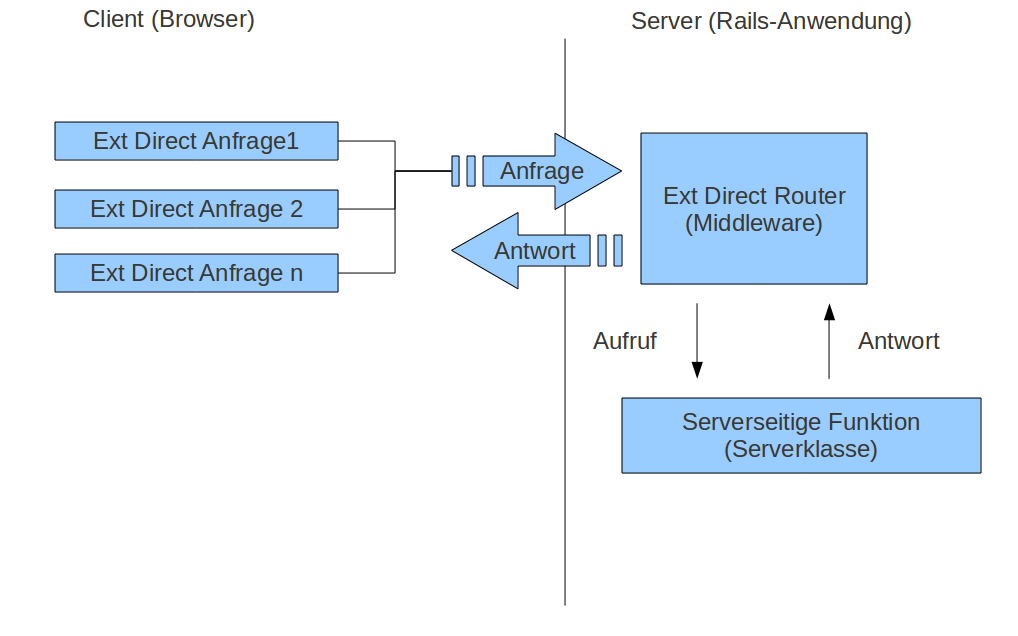
\includegraphics[scale=0.55]{images/rack/extdirect.png}
\caption{Schema des Ext Direct Routing mit \emph{extr}}
\end{center}
\end{figure}

Die Installation und Nutzung der Erweiterung \emph{extr} wird im Anhang dieser Arbeit demonstriert. Auf Grund des frühen Entwicklungsstatus unterstützt die Erweiterung serverseitig noch nicht alle der geforderten Ext-Direct-Funktionalitäten. Im folgenden sollen bestehende Beschränkungen und Probleme erläutert werden:
\begin{itemize}
\item
Ext Direct-Anfragen mit Parametern aus Formularen und Datei-Uploads (Form Posts) werden von der Rails Middleware noch nicht vollständig an die entsprechende Zielmethode (controller action) weitergeleitet.
\item
kein Schutz vor CSRF/XSRF-Angriffen\footnote{\href{http://guides.rubyonrails.org/security.html\#cross-site-request-forgery-csrf}{http://guides.rubyonrails.org/security.html\#cross-site-request-forgery-csrf}}
\end{itemize}

